\lhead{\emph{Capitolo 4}}
\chapter{Conclusioni}

In questo capitolo si illustreranno quali sono stati i risultati del lavoro svolto e con le opportune valutazioni e commenti. Per confrontare i risultati dello sviluppo multi piattaforma con il modello ibrido, si farà riferimento ai tempi di sviluppo e alla qualità del software prodotto. Inoltre si illustrerà qual'è il trend attuale del mercato delle applicazioni e dei dispositivi mobili, per valutare la scelta delle tecnologie per lo sviluppo. Inoltre si faranno riferimenti a tecnologie web emergenti legate al campo dello sviluppo multi piattaforma.

\section{I cambiamenti sul processo di sviluppo}
Nello sviluppo di una applicazione in generale, tutte le figure professionali coinvolte fanno riferimento ad uno schema generale, che illustra le fasi di lavoro per arrivare al prodotto finale. Da quanto appreso durante l'esperienza di tirocinio in azienda, questo schema deve essere il più generico possibile, e comprensibile da chiunque lavori con esso. Nella figura \ref{fig:classic_app_flow} si possono osservare le fasi principali dello sviluppo di una applicazione.

\begin{figure}
	\begin{center}
		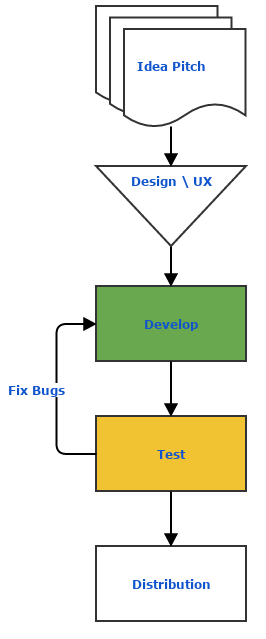
\includegraphics[scale=0.5]{Figures/classic_app_flow.png}
		\caption[Schema generale]{In questo schema sono illustrate le fasi generiche dello sviluppo di una applicazione}
		\label{fig:classic_app_flow}
	\end{center}
\end{figure}

Durante la mia esperienza ho ricoperto il ruolo di sviluppatore frontend, quindi mi sono occupato delle fasi di sviluppo e di test. Generalmente il lavoro viene svolto in team dove le competenze professionali sono omogenee e ognuno e dedico ad una sezione specifica dello schema.

Prendendo spunto da questo schema generale ho creato una espansione della fase di sviluppo e di test per lo sviluppo di applicazioni multipiattaforma ibride. Si tratta di un sottoschema che evidenzia quali fasi hanno caratterizzato un primo approccio a questo tipo di sviluppo.
Una prima fase è stata quella di scegliere quali tecnologie web utilizzare per lo sviluppo ibrido, e quali per per testare il codice che doveva essere prodotto. Nel mio caso il framework AnagularJS si prestava già ad uno sviluppo di questo tipo e non ho impiegato molto tempo nel capire come utilizzarlo per lo sviluppo mobile. In altri casi, data la vasta scelta di framework javascript per lo sviluppo mobile, la scelta può richiedere parecchio tempo(dipende dalle competenze e dallo stile del programmatore).
Dopo aver costruito il mio ambiente di sviluppo ho proceduto come nello schema \ref{fig:classic_app_flow} sviluppando e testando l'applicazione.

Certamente iterare questo processo per ciascuna applicazione che si andrà a sviluppare è molto dispendioso in termini di tempo e risorse. Una buona soluzione e costruirsi un set di tecnologie che si andranno a utilizzare per lo sviluppo di ciascuna applicazione futura, quello che in azienda si è chiamato \emph{skeleton}. Ovviamente lo scheletro di una applicazione tipo deve essere fatto in modo da espandersi nel caso giungessero richieste di caratteristiche non ancora incluse. Nella figura \ref{fig:flow_match} si può osservare l'evoluzione del primo schema verso una soluzione pronta e rapida all'utilizzo.

\begin{figure}
	\begin{center}
		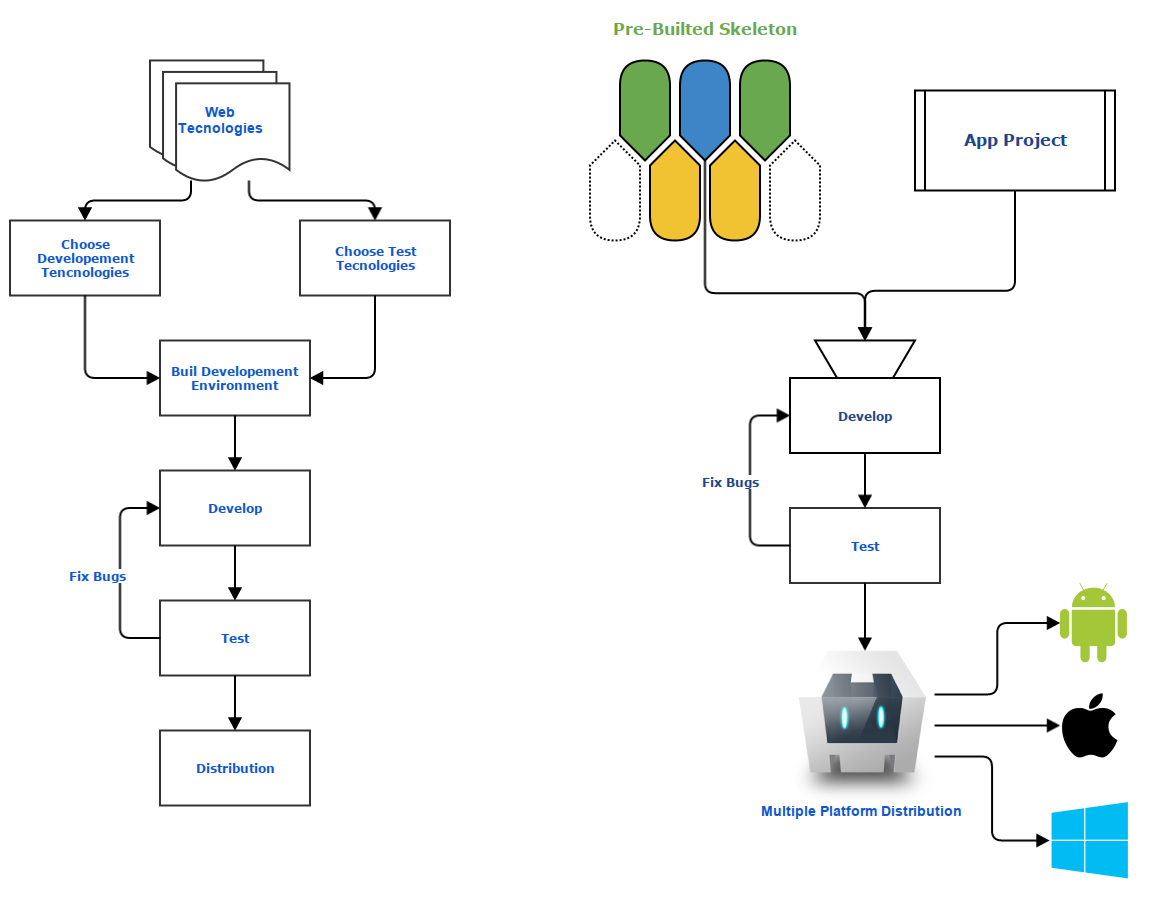
\includegraphics[scale=0.5]{Figures/match_flow.png}
		\caption[Schemi di sviluppo a confronto]{Questo schema illustra l'evoluzione del primo schema verso una struttura più completa e multipiattaforma}
		\label{fig:flow_match}
	\end{center}
\end{figure}

Il mio ruolo di sviluppatore web è stato proprio quello di tradurre le richieste del cliente all'interno dello scheletro di applicazione, fornitomi dall'azienda. Partendo da questo modello, l'ho evoluto aggiungendogli la possibilità di essere multipiattaforma.


\section{Considerazioni sullo sviluppo ibrido}

\subsection{Quando conviene lo sviluppo ibrido}

\subsection{Le tecnologie web, molto di più dei semplici framework}

\section{Risultati sulle tecnologie utilizzate}

-- Vantaggi-- \\
-- Criticità --\\


\section{Ciclo di vita di una app}
-- Statistiche sulle app\\
	-- Stessa App replicata nei store --\\
	-- Durata delle app --\\
-- Aggiornamenti --\\
	-- più piattaforme = più aggiornamenti --\\
-- Mantenimento --\\
	-- Aggiornamento delle versioni --\\
	-- Debug --\\
-- Tutto ovviamente in confronto con lo sviluppo ibrido --

\section{L'aspetto commerciale e le possibili soluzioni}

-- Come può un azienda adottare soluzioni cross platform --\\
-- Azienda\\
	-- Tipi di app sviluppate\\
	-- Approccio ibrido oppure no\\
	-- Scelta in base alla natura delle app

\section{Nuove tecnologie web emergenti}

\subsection{FirefoxOS}

\subsection{WebOS}

\subsection{Node Webkit}